
\subsubsection{Exascale Code Generation Toolkit} 


\paragraph{Overview} 

Our project addresses the development of HPC software for exascale and similarly complex architectures. 
Generated code 
may be modified, wrapped in application specific APIs, or be checked into the user’s application 
repository. Inputs to the code generation tools we have developed are either application 
code or simplified application code that represents naive implementations of algorithms. Input languages 
we are supporting include both legacy and modern versions of Fortran, C, and C++ 
(e.g., F77, F2008, F2015, C89, C99, C11, C++98, C++11, C++14, C++17, etc.). The output is generated 
code in the same language, but modified to address essential hardware-specific architectural features. 
We are supporting common language dialects including: UPC, OpenMP 
(for both C, C++, and Fortran), CUDA, and OpenCL.

\paragraph{Key  Challenges}

   Our project addresses the development of HPC software for exascale and
similarly complex architectures.
The approach in our project supports only the generation of code to simplify 
the job of the developers, and as such 
users are given complete control over how to use our code generation tools.
However, this makes our project especially difficult because we must read and rewrite 
the user's source code application.  This step requires significant compiler technology: 
analysis and transformations at the source code level so that it can leverage the vendor's compiler.
% Generated code may be modified, wrapped in application specific APIs, or be checked 
% into the user's application repository. 

We operate using a source-to-source approach so that the target architecture's compiler 
(vendor compiler) may be used to full advantage. It is expected that the vendor's compiler 
will be best optimized (low level optimizations) to the vendor's architecture. However, 
the structure of code written (at a high level) to take advantage of the vendor compiler's 
optimization can be exceedingly complex, vary widely between vendors, and is thus well 
better suited to automated code generation.

\paragraph{Solution Strategy}


Figure~\ref{fig:2.3.2.05-ExascaleCodeGenToolkit} illustrates the approach used to process 
application code and automate transformations to support either performance optimization 
or correctness checking.
\begin{figure}[htb]
	\centering
	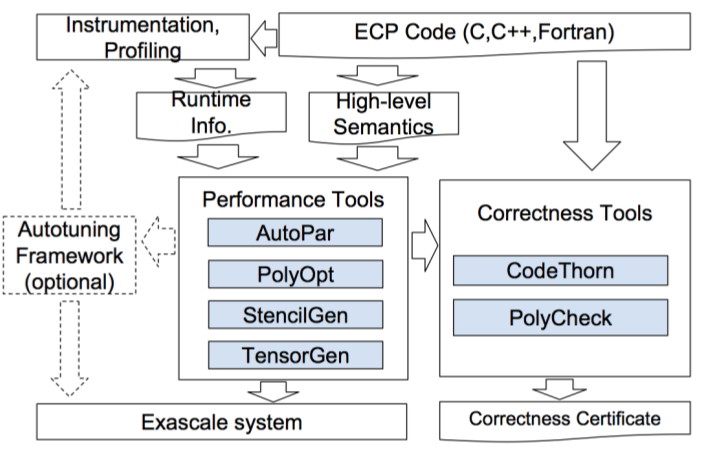
\includegraphics[width=4.5in]{projects/2.3.2-Tools/2.3.2.05-Exascale-Code-Generation-Toolkit/ExascaleCodeGenToolkit.png}
	\caption{\label{fig:2.3.2.05-ExascaleCodeGenToolkit} Approach to processing user application 
                 code with multiple tools to support optimization and correctness checking.}
\end{figure}
Our project is developing several tools for generating code: PolyOpt (a polyhedral 
optimizations program transformation engine capable of fully automating highly complex loop transformations), 
AutoPar (an automatic parallelization tool that inserts OpenMP directives into serial codes), 
CodeThorn (an award winning code correctness tool built using ROSE and SPOT),  PolyCheck (a code 
correctness tool specific to polyhedral optimizations), and ROSE (a widely used compiler infrastructure 
for building specialized compiler tools). Our tools allow users to easily specify portions of an input application and 
automatically generate semantically equivalent, but higher performing code variants; including the ability 
to generate a multiple variants that traverse a space of optimizations (e.g., loop tiling sizes, loop fusion, 
loop fission alternatives, etc.). The PolyOpt polyhedral optimizer is being enhanced with pattern-specific 
optimization and code generation strategies to address important patterns found in ECP codes. Stand-alone 
code generators developed previously by us for stencil computations and tensor contractions are being 
integrated with PolyOpt and their capabilities enhanced and hardened (StencilGen and TensorGen).  The 
use of CodeThorn and PolyCheck have already been demonstrated for the verification of correctness of 
such automatically generated code.

\paragraph{Recent Progress}

We have made a release of TensorGen to the NWChem team and it has been used in their NWChem production 
release this past Fall (Fall 2017).

The StencilGen code generator takes as input a DSL specification of stencil functions and their domains, and 
creates CUDA code from it. The tool employs fusion, streaming, and overlapped tiling to achieve high performance. 
In order to avoid register spills for complex stencils, the tool also performs statement reordering that takes as 
input straight-line CUDA code for a multi-statement stencil and models it as a DAG of expression trees. The 
statements are then reordered to minimize register pressure \cite{PPoPP18}.

The AutoPar tool accepts C/C++ serial programs as input and automatically generates OpenMP loop directives. We 
have continued to work on the CPU cost model to guide AutoPar’s automatic parallelization. We have created a model 
based on the roofline model, and an existing tool in ROSE (the Arithmetic intensity tool) has been improved to 
provide key information for our model. We also added one option to use inlining in order to support loops with 
simple C function calls.  Several microbenchmarks, including EPCC and STREAM, have been investigated and used 
to extract hardware and software metrics needed in our model.

CodeThorn takes as input polyhedral parallelized loops generated by the tool PolyOpt and checks whether the 
optimized loops are equivalent to the original (non-optimized) loops. We analyzed the availability of optimizable 
code patterns for verification in three proxy apps (AMG2013, CoMD, LULESH) and found 282 optimizable patterns 
that can serve as input to our verification. We extended the scope of the covered C++ subset for verification 
to support changes in the PolyOpt generated optimized code. We also extended the representation of program states 
to take pointers to dynamic data structures into account.

We have been developing the other tools mentioned above, adding supporting features, and testing to them.
We gave a demo of these tools at the recent ECP all-hands meeting in February, 2018; and we distribute 
the working versions of these tools that we demonstrated at the meeting.  These tools are regularly updated 
with ongoing work and released as part of Continuous Integration (CI) processes.  Most tools are released
as part of the ROSE distribution to simplify the testing and release process.

We have been adding new Fortran support to ROSE as part of our ECP Fortran support. We have also started 
the C++17 support in ROSE. We have compiled most of the ECP proxy applications as part of initial first 
year work. We now test the ROSE C and C++ compiler infrastructure against commercial compiler tests suits
and it performs similarly to commercial compilers in initial testing for analysis tools.



\paragraph{Next Steps}

For StencilGen, we will develop several heuristics for fusion, streaming, and tiling based on architectural 
characteristics, as well as machinery to systematically explore various compositions of optimizations and 
optimization parameters. We will continue to work with the NWChem team at PNNL to support their computational 
code generation requirements.
For CodeThorn we will (i) extend the evaluation with proxy apps and (ii) improve the reporting of detected 
semantic differences in the PolyOpt optimized code in comparison to the original code.

We are also working with the AMReX ECP team to support analysis and transformation of their application codes
using our tools and future versions of them with additional features.  The AMReX team is in turn also 
supporting multiple ECP application teams, to which all of our work is expected to apply directly.


 

